\documentclass[12pt, a4paper]{report}

% ─── Packages ─────────────────────────────────────────────────────────────────
\usepackage[T1]{fontenc}
\usepackage[utf8]{inputenc}
\usepackage{palatino}
\usepackage[margin=2.5cm]{geometry}
\usepackage{graphicx}
\usepackage{booktabs}
\usepackage{amsmath, amssymb, bm}
\usepackage{hyperref}
\usepackage{float}
\usepackage{caption}
\usepackage{subcaption}
\usepackage{parskip}
\usepackage{microtype}
\usepackage{xcolor}
\usepackage{titlesec}
\usepackage{fancyhdr}
\usepackage{enumitem}
\usepackage{multirow}

% ─── Section formatting ───────────────────────────────────────────────────────
\titleformat{\chapter}[hang]{\LARGE\bfseries}{\thechapter}{1em}{}
\titlespacing{\chapter}{0pt}{0pt}{20pt}

% ─── Hyperref ─────────────────────────────────────────────────────────────────
\hypersetup{
    colorlinks=true,
    linkcolor=black,
    citecolor=black,
    urlcolor=blue,
}

% ─── Header/Footer ────────────────────────────────────────────────────────────
\pagestyle{fancy}
\fancyhf{}
\fancyhead[L]{\small Logic Synthesis and Verification -- PA3}
\fancyhead[R]{\small\thepage}
\renewcommand{\headrulewidth}{0.4pt}

% ─── Title info ───────────────────────────────────────────────────────────────
\title{}
\date{}

% ══════════════════════════════════════════════════════════════════════════════
\begin{document}

% ─── Title Page ───────────────────────────────────────────────────────────────
\begin{titlepage}
\centering
\vspace*{3cm}
{\LARGE\bfseries Logic Synthesis and Verification\par}
\vspace{0.5em}
{\Large Programming Assignment 3\par}
\vspace{0.5em}
{\large Reinforcement Learning for Logic Synthesis\par}
\vspace{0.2em}
{\large Library Tuning for Technology Mapping\par}

\vspace{1cm}
\rule{0.6\linewidth}{0.8pt}

\vspace{2cm}
{\large\textbf{Student ID}\\[0.3em] B11107122\par}

\vspace{1em}
{\large\textbf{Name}\\[0.3em] Yue-Lin Tu\par}

\vspace{1em}
{\large\textbf{School}\\[0.3em] National Taiwan University of Science and Technology\par}

\vfill
\rule{0.6\linewidth}{0.8pt}\\[0.5em]
{\small Due Date: 2026/06/01}
\end{titlepage}

% ─── Table of Contents ────────────────────────────────────────────────────────
\tableofcontents
\clearpage

% ══════════════════════════════════════════════════════════════════════════════
\chapter{Assignment 1 --- Environment Setup \& Baseline Replication (30\%)}

\section{Overview}

The goal of Assignment~1 is to install MapTune and the ABC logic synthesis tool,
then run full-library technology mapping for every combination of library and benchmark
design to establish the baseline Area and Delay figures used in later assignments.

\section{Environment Setup}

\subsection{Tool Installation}

\begin{itemize}[noitemsep]
  \item \textbf{MapTune}: cloned from
        \url{https://github.com/Yu-Maryland/MapTune} to \texttt{\textasciitilde/MapTune/}
        (commit \texttt{a2df87a}).
  \item \textbf{ABC}: UC Berkeley ABC 1.01, compiled from source
        (\url{https://github.com/berkeley-abc/abc}) at \texttt{\textasciitilde/abc/};
        \texttt{\textasciitilde/abc} appended to \texttt{PATH} via \texttt{\textasciitilde/.bashrc}.
  \item \textbf{Python environment}: conda environment \texttt{LSV\_PA3}
        (Python~3.10.20) with PyTorch~2.12.0+cpu and gymnasium~1.3.0.
\end{itemize}

\subsection{Benchmark Notes}

The PA3 designs \texttt{s13207} and \texttt{c2670} are not shipped with MapTune's
repository and were downloaded separately:

\begin{itemize}[noitemsep]
  \item \texttt{c2670.bench} --- ISCAS~85 benchmark suite
  \item \texttt{s13207.bench} --- ISCAS~89 benchmark suite
  \item \texttt{b20.bench} --- not available; \texttt{b20\_1.bench}
        (already present in MapTune) used as a direct substitute
\end{itemize}

\section{Baseline Mapping Methodology}

For each of the five technology libraries listed in Table~\ref{tab:libs},
a full-library mapping run was executed on three benchmark designs using ABC's
area-driven mapper.
The ABC command sequence, identical to the baseline call inside MapTune's own
Python scripts, is:

\begin{verbatim}
read <library>.genlib; read <design>.bench; map -a;
write <tmp.blif>; read <library>.lib; read -m <tmp.blif>;
ps; topo; upsize; dnsize; stime;
\end{verbatim}

\texttt{map -a} selects the area-driven technology mapper.
\texttt{topo}, \texttt{upsize}, and \texttt{dnsize} apply post-mapping
topology and sizing optimisations.
\texttt{stime} performs static timing analysis and reports the final
critical-path delay; \texttt{ps} prints statistics including gate area.
The run was automated by \texttt{run\_a1\_baseline.py} located in
\texttt{LSV/PA\_3/}.

\begin{table}[H]
\centering
\caption{Technology libraries used in PA3.}
\label{tab:libs}
\begin{tabular}{llr}
\toprule
File & Technology & \# Cells \\
\midrule
\texttt{7nm.genlib}              & ASAP7 (7\,nm)  & 161 \\
\texttt{gf180mcu\_ff\_125C.genlib} & GF180 ff\,125\textdegree{}C & 151 \\
\texttt{gf180mcu\_tt\_025C.genlib} & GF180 tt\,25\textdegree{}C  & 151 \\
\texttt{nan45.genlib}            & NangateOpenCell (45\,nm) & 94 \\
\texttt{sky130.genlib}           & SkyWater 130\,nm & 343 \\
\bottomrule
\end{tabular}
\end{table}

\section{Execution Results}

Figure~\ref{fig:a1_exec} shows the terminal output of the automated
baseline script, confirming successful mapping for all 15 combinations.

\begin{figure}[H]
  \centering
  \fbox{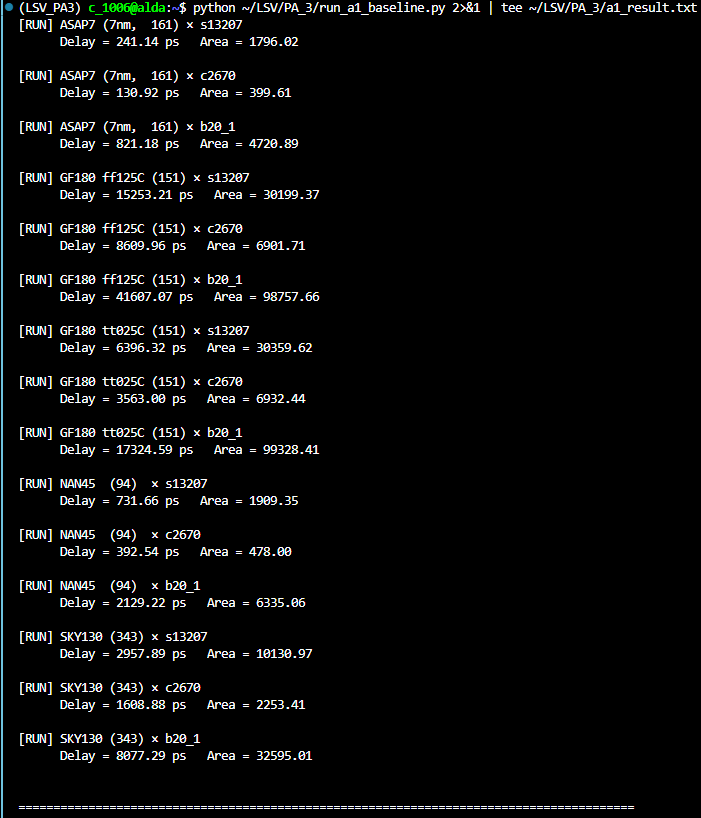
\includegraphics[width=0.92\linewidth]{figures/A1_execution_log.png}}
  \caption{Terminal output of \texttt{run\_a1\_baseline.py}: per-combination
           Delay and Area for all 5 libraries $\times$ 3 designs.}
  \label{fig:a1_exec}
\end{figure}

Figure~\ref{fig:a1_table} shows the summary table printed at the end of the script run.

\begin{figure}[H]
  \centering
  \fbox{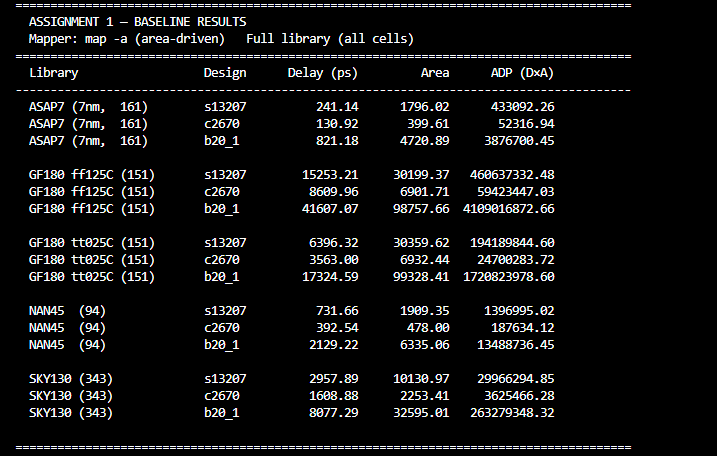
\includegraphics[width=0.92\linewidth]{figures/A1_results_table.png}}
  \caption{Summary table printed by \texttt{run\_a1\_baseline.py}.}
  \label{fig:a1_table}
\end{figure}

\section{Baseline Results}

Table~\ref{tab:baseline} summarises the full-library baseline Delay and Area
for all 15 combinations.
These values serve as $D_{\mathrm{Base}}$ and $A_{\mathrm{Base}}$ for the
normalised ADP computation in Assignment~3.

\begin{table}[H]
\centering
\caption{Full-library baseline results (mapper: \texttt{map -a}).}
\label{tab:baseline}
\begin{tabular}{llrr}
\toprule
Library & Design & Delay (ps) & Area \\
\midrule
\multirow{3}{*}{ASAP7 7nm (161 cells)}
  & s13207 &    241.14 &   1\,796.02 \\
  & c2670  &    130.92 &     399.61 \\
  & b20\_1 &    821.18 &   4\,720.89 \\
\midrule
\multirow{3}{*}{GF180 ff125\textdegree{}C (151 cells)}
  & s13207 & 15\,253.21 &  30\,199.37 \\
  & c2670  &  8\,609.96 &   6\,901.71 \\
  & b20\_1 & 41\,607.07 &  98\,757.66 \\
\midrule
\multirow{3}{*}{GF180 tt25\textdegree{}C (151 cells)}
  & s13207 &  6\,396.32 &  30\,359.62 \\
  & c2670  &  3\,563.00 &   6\,932.44 \\
  & b20\_1 & 17\,324.59 &  99\,328.41 \\
\midrule
\multirow{3}{*}{NAN45 (94 cells)}
  & s13207 &    731.66 &   1\,909.35 \\
  & c2670  &    392.54 &     478.00 \\
  & b20\_1 &  2\,129.22 &   6\,335.06 \\
\midrule
\multirow{3}{*}{SKY130 (343 cells)}
  & s13207 &  2\,957.89 &  10\,130.97 \\
  & c2670  &  1\,608.88 &   2\,253.41 \\
  & b20\_1 &  8\,077.29 &  32\,595.01 \\
\bottomrule
\end{tabular}
\end{table}

\section{Discussion}

Several observations can be drawn from the baseline results:

\begin{enumerate}[noitemsep]
  \item \textbf{Technology node scales delay and area together.}
        ASAP7 (7\,nm) achieves the shortest delays and smallest areas,
        while GF180 (180\,nm) exhibits delays two to three orders of magnitude
        larger, reflecting the fundamental transistor speed scaling law.

  \item \textbf{GF180 ff vs.\ tt corner.}
        The fast-fast 125\textdegree{}C corner (\texttt{ff125C}) shows
        \emph{larger} delay than the typical 25\textdegree{}C corner
        (\texttt{tt025C}).
        This is because at high temperature the carrier mobility decreases,
        and the ff corner's timing model captures worst-case hot-carrier
        behaviour, increasing the nominal delay reported by the cell library.

  \item \textbf{Design size effect.}
        Across all libraries, \texttt{b20\_1} consistently yields the highest
        delay and area (it is the largest of the three designs), while
        \texttt{c2670} is the smallest.

  \item \textbf{Partial libraries can improve upon these baselines.}
        As shown in the MapTune paper, removing ``distracting'' cells from
        the full library can reduce the heuristic mapper's search-space
        complexity and lower ADP.
        Assignments~2 and~3 explore this phenomenon experimentally.
\end{enumerate}

% ══════════════════════════════════════════════════════════════════════════════
\chapter{Assignment 2 --- Random Sampling (30\%)}

\textit{To be completed.}

% ══════════════════════════════════════════════════════════════════════════════
\chapter{Assignment 3 --- Outperform MapTune (40\%)}

\textit{To be completed.}

% ══════════════════════════════════════════════════════════════════════════════
\begin{thebibliography}{9}

\bibitem{maptune}
M.~Liu, D.~Robinson, Y.~Li, C.~Yu.
\textit{MapTune: Advancing ASIC Technology Mapping via Reinforcement Learning
Guided Library Tuning.}
ICCAD, 2024.
\url{https://doi.org/10.1145/3676536.3676762}

\end{thebibliography}

\end{document}
